
%% bare_jrnl.tex
%% V1.4b
%% 2015/08/26
%% by Michael Shell
%% see http://www.michaelshell.org/
%% for current contact information.
%%
%% This is a skeleton file demonstrating the use of IEEEtran.cls
%% (requires IEEEtran.cls version 1.8b or later) with an IEEE
%% journal paper.
%%
%% Support sites:
%% http://www.michaelshell.org/tex/ieeetran/
%% http://www.ctan.org/pkg/ieeetran
%% and
%% http://www.ieee.org/

%%*************************************************************************
%% Legal Notice:
%% This code is offered as-is without any warranty either expressed or
%% implied; without even the implied warranty of MERCHANTABILITY or
%% FITNESS FOR A PARTICULAR PURPOSE! 
%% User assumes all risk.
%% In no event shall the IEEE or any contributor to this code be liable for
%% any damages or losses, including, but not limited to, incidental,
%% consequential, or any other damages, resulting from the use or misuse
%% of any information contained here.
%%
%% All comments are the opinions of their respective authors and are not
%% necessarily endorsed by the IEEE.
%%
%% This work is distributed under the LaTeX Project Public License (LPPL)
%% ( http://www.latex-project.org/ ) version 1.3, and may be freely used,
%% distributed and modified. A copy of the LPPL, version 1.3, is included
%% in the base LaTeX documentation of all distributions of LaTeX released
%% 2003/12/01 or later.
%% Retain all contribution notices and credits.
%% ** Modified files should be clearly indicated as such, including  **
%% ** renaming them and changing author support contact information. **
%%*************************************************************************


% *** Authors should verify (and, if needed, correct) their LaTeX system  ***
% *** with the testflow diagnostic prior to trusting their LaTeX platform ***
% *** with production work. The IEEE's font choices and paper sizes can   ***
% *** trigger bugs that do not appear when using other class files.       ***                          ***
% The testflow support page is at:
% http://www.michaelshell.org/tex/testflow/



\documentclass[journal]{IEEEtran}
%
% If IEEEtran.cls has not been installed into the LaTeX system files,
% manually specify the path to it like:
% \documentclass[journal]{../sty/IEEEtran}


\usepackage{hyperref}


% Some very useful LaTeX packages include:
% (uncomment the ones you want to load)


% *** MISC UTILITY PACKAGES ***
%
%\usepackage{ifpdf}
% Heiko Oberdiek's ifpdf.sty is very useful if you need conditional
% compilation based on whether the output is pdf or dvi.
% usage:
% \ifpdf
%   % pdf code
% \else
%   % dvi code
% \fi
% The latest version of ifpdf.sty can be obtained from:
% http://www.ctan.org/pkg/ifpdf
% Also, note that IEEEtran.cls V1.7 and later provides a builtin
% \ifCLASSINFOpdf conditional that works the same way.
% When switching from latex to pdflatex and vice-versa, the compiler may
% have to be run twice to clear warning/error messages.






% *** CITATION PACKAGES ***
%
%\usepackage{cite}
% cite.sty was written by Donald Arseneau
% V1.6 and later of IEEEtran pre-defines the format of the cite.sty package
% \cite{} output to follow that of the IEEE. Loading the cite package will
% result in citation numbers being automatically sorted and properly
% "compressed/ranged". e.g., [1], [9], [2], [7], [5], [6] without using
% cite.sty will become [1], [2], [5]--[7], [9] using cite.sty. cite.sty's
% \cite will automatically add leading space, if needed. Use cite.sty's
% noadjust option (cite.sty V3.8 and later) if you want to turn this off
% such as if a citation ever needs to be enclosed in parenthesis.
% cite.sty is already installed on most LaTeX systems. Be sure and use
% version 5.0 (2009-03-20) and later if using hyperref.sty.
% The latest version can be obtained at:
% http://www.ctan.org/pkg/cite
% The documentation is contained in the cite.sty file itself.






% *** GRAPHICS RELATED PACKAGES ***
%
\usepackage{graphicx}
\ifCLASSINFOpdf
  % \usepackage[pdftex]{graphicx}
  % declare the path(s) where your graphic files are
  % \graphicspath{{../pdf/}{../jpeg/}}
  % and their extensions so you won't have to specify these with
  % every instance of \includegraphics
  % \DeclareGraphicsExtensions{.pdf,.jpeg,.png}
\else
  % or other class option (dvipsone, dvipdf, if not using dvips). graphicx
  % will default to the driver specified in the system graphics.cfg if no
  % driver is specified.
  % \usepackage[dvips]{graphicx}
  % declare the path(s) where your graphic files are
  % \graphicspath{{../eps/}}
  % and their extensions so you won't have to specify these with
  % every instance of \includegraphics
  % \DeclareGraphicsExtensions{.eps}
\fi
% graphicx was written by David Carlisle and Sebastian Rahtz. It is
% required if you want graphics, photos, etc. graphicx.sty is already
% installed on most LaTeX systems. The latest version and documentation
% can be obtained at: 
% http://www.ctan.org/pkg/graphicx
% Another good source of documentation is "Using Imported Graphics in
% LaTeX2e" by Keith Reckdahl which can be found at:
% http://www.ctan.org/pkg/epslatex
%
% latex, and pdflatex in dvi mode, support graphics in encapsulated
% postscript (.eps) format. pdflatex in pdf mode supports graphics
% in .pdf, .jpeg, .png and .mps (metapost) formats. Users should ensure
% that all non-photo figures use a vector format (.eps, .pdf, .mps) and
% not a bitmapped formats (.jpeg, .png). The IEEE frowns on bitmapped formats
% which can result in "jaggedy"/blurry rendering of lines and letters as
% well as large increases in file sizes.
%
% You can find documentation about the pdfTeX application at:
% http://www.tug.org/applications/pdftex





% *** MATH PACKAGES ***
%
\usepackage{amsfonts}
%\usepackage{amsmath}
% A popular package from the American Mathematical Society that provides
% many useful and powerful commands for dealing with mathematics.
%
% Note that the amsmath package sets \interdisplaylinepenalty to 10000
% thus preventing page breaks from occurring within multiline equations. Use:
%\interdisplaylinepenalty=2500
% after loading amsmath to restore such page breaks as IEEEtran.cls normally
% does. amsmath.sty is already installed on most LaTeX systems. The latest
% version and documentation can be obtained at:
% http://www.ctan.org/pkg/amsmath





% *** SPECIALIZED LIST PACKAGES ***
%
%\usepackage{algorithmic}
% algorithmic.sty was written by Peter Williams and Rogerio Brito.
% This package provides an algorithmic environment fo describing algorithms.
% You can use the algorithmic environment in-text or within a figure
% environment to provide for a floating algorithm. Do NOT use the algorithm
% floating environment provided by algorithm.sty (by the same authors) or
% algorithm2e.sty (by Christophe Fiorio) as the IEEE does not use dedicated
% algorithm float types and packages that provide these will not provide
% correct IEEE style captions. The latest version and documentation of
% algorithmic.sty can be obtained at:
% http://www.ctan.org/pkg/algorithms
% Also of interest may be the (relatively newer and more customizable)
% algorithmicx.sty package by Szasz Janos:
% http://www.ctan.org/pkg/algorithmicx




% *** ALIGNMENT PACKAGES ***
%
%\usepackage{array}
% Frank Mittelbach's and David Carlisle's array.sty patches and improves
% the standard LaTeX2e array and tabular environments to provide better
% appearance and additional user controls. As the default LaTeX2e table
% generation code is lacking to the point of almost being broken with
% respect to the quality of the end results, all users are strongly
% advised to use an enhanced (at the very least that provided by array.sty)
% set of table tools. array.sty is already installed on most systems. The
% latest version and documentation can be obtained at:
% http://www.ctan.org/pkg/array


% IEEEtran contains the IEEEeqnarray family of commands that can be used to
% generate multiline equations as well as matrices, tables, etc., of high
% quality.




% *** SUBFIGURE PACKAGES ***
%\ifCLASSOPTIONcompsoc
%  \usepackage[caption=false,font=normalsize,labelfont=sf,textfont=sf]{subfig}
%\else
%  \usepackage[caption=false,font=footnotesize]{subfig}
%\fi
% subfig.sty, written by Steven Douglas Cochran, is the modern replacement
% for subfigure.sty, the latter of which is no longer maintained and is
% incompatible with some LaTeX packages including fixltx2e. However,
% subfig.sty requires and automatically loads Axel Sommerfeldt's caption.sty
% which will override IEEEtran.cls' handling of captions and this will result
% in non-IEEE style figure/table captions. To prevent this problem, be sure
% and invoke subfig.sty's "caption=false" package option (available since
% subfig.sty version 1.3, 2005/06/28) as this is will preserve IEEEtran.cls
% handling of captions.
% Note that the Computer Society format requires a larger sans serif font
% than the serif footnote size font used in traditional IEEE formatting
% and thus the need to invoke different subfig.sty package options depending
% on whether compsoc mode has been enabled.
%
% The latest version and documentation of subfig.sty can be obtained at:
% http://www.ctan.org/pkg/subfig




% *** FLOAT PACKAGES ***
%
%\usepackage{fixltx2e}
% fixltx2e, the successor to the earlier fix2col.sty, was written by
% Frank Mittelbach and David Carlisle. This package corrects a few problems
% in the LaTeX2e kernel, the most notable of which is that in current
% LaTeX2e releases, the ordering of single and double column floats is not
% guaranteed to be preserved. Thus, an unpatched LaTeX2e can allow a
% single column figure to be placed prior to an earlier double column
% figure.
% Be aware that LaTeX2e kernels dated 2015 and later have fixltx2e.sty's
% corrections already built into the system in which case a warning will
% be issued if an attempt is made to load fixltx2e.sty as it is no longer
% needed.
% The latest version and documentation can be found at:
% http://www.ctan.org/pkg/fixltx2e


%\usepackage{stfloats}
% stfloats.sty was written by Sigitas Tolusis. This package gives LaTeX2e
% the ability to do double column floats at the bottom of the page as well
% as the top. (e.g., "\begin{figure*}[!b]" is not normally possible in
% LaTeX2e). It also provides a command:
%\fnbelowfloat
% to enable the placement of footnotes below bottom floats (the standard
% LaTeX2e kernel puts them above bottom floats). This is an invasive package
% which rewrites many portions of the LaTeX2e float routines. It may not work
% with other packages that modify the LaTeX2e float routines. The latest
% version and documentation can be obtained at:
% http://www.ctan.org/pkg/stfloats
% Do not use the stfloats baselinefloat ability as the IEEE does not allow
% \baselineskip to stretch. Authors submitting work to the IEEE should note
% that the IEEE rarely uses double column equations and that authors should try
% to avoid such use. Do not be tempted to use the cuted.sty or midfloat.sty
% packages (also by Sigitas Tolusis) as the IEEE does not format its papers in
% such ways.
% Do not attempt to use stfloats with fixltx2e as they are incompatible.
% Instead, use Morten Hogholm'a dblfloatfix which combines the features
% of both fixltx2e and stfloats:
%
% \usepackage{dblfloatfix}
% The latest version can be found at:
% http://www.ctan.org/pkg/dblfloatfix




%\ifCLASSOPTIONcaptionsoff
%  \usepackage[nomarkers]{endfloat}
% \let\MYoriglatexcaption\caption
% \renewcommand{\caption}[2][\relax]{\MYoriglatexcaption[#2]{#2}}
%\fi
% endfloat.sty was written by James Darrell McCauley, Jeff Goldberg and 
% Axel Sommerfeldt. This package may be useful when used in conjunction with 
% IEEEtran.cls'  captionsoff option. Some IEEE journals/societies require that
% submissions have lists of figures/tables at the end of the paper and that
% figures/tables without any captions are placed on a page by themselves at
% the end of the document. If needed, the draftcls IEEEtran class option or
% \CLASSINPUTbaselinestretch interface can be used to increase the line
% spacing as well. Be sure and use the nomarkers option of endfloat to
% prevent endfloat from "marking" where the figures would have been placed
% in the text. The two hack lines of code above are a slight modification of
% that suggested by in the endfloat docs (section 8.4.1) to ensure that
% the full captions always appear in the list of figures/tables - even if
% the user used the short optional argument of \caption[]{}.
% IEEE papers do not typically make use of \caption[]'s optional argument,
% so this should not be an issue. A similar trick can be used to disable
% captions of packages such as subfig.sty that lack options to turn off
% the subcaptions:
% For subfig.sty:
% \let\MYorigsubfloat\subfloat
% \renewcommand{\subfloat}[2][\relax]{\MYorigsubfloat[]{#2}}
% However, the above trick will not work if both optional arguments of
% the \subfloat command are used. Furthermore, there needs to be a
% description of each subfigure *somewhere* and endfloat does not add
% subfigure captions to its list of figures. Thus, the best approach is to
% avoid the use of subfigure captions (many IEEE journals avoid them anyway)
% and instead reference/explain all the subfigures within the main caption.
% The latest version of endfloat.sty and its documentation can obtained at:
% http://www.ctan.org/pkg/endfloat
%
% The IEEEtran \ifCLASSOPTIONcaptionsoff conditional can also be used
% later in the document, say, to conditionally put the References on a 
% page by themselves.




% *** PDF, URL AND HYPERLINK PACKAGES ***
%
%\usepackage{url}
% url.sty was written by Donald Arseneau. It provides better support for
% handling and breaking URLs. url.sty is already installed on most LaTeX
% systems. The latest version and documentation can be obtained at:
% http://www.ctan.org/pkg/url
% Basically, \url{my_url_here}.


\usepackage{color}
\usepackage[dvipsnames]{xcolor}
\usepackage{soul}

% *** Do not adjust lengths that control margins, column widths, etc. ***
% *** Do not use packages that alter fonts (such as pslatex).         ***
% There should be no need to do such things with IEEEtran.cls V1.6 and later.
% (Unless specifically asked to do so by the journal or conference you plan
% to submit to, of course. )


% correct bad hyphenation here
\hyphenation{op-tical net-works semi-conduc-tor ns- however}


\begin{document}
%
% paper title
% Titles are generally capitalized except for words such as a, an, and, as,
% at, but, by, for, in, nor, of, on, or, the, to and up, which are usually
% not capitalized unless they are the first or last word of the title.
% Linebreaks \\ can be used within to get better formatting as desired.
% Do not put math or special symbols in the title.
\title{A Flexible Machine Learning-Aware Architecture\\ for Future WLANs}
%
%
% author names and IEEE memberships
% note positions of commas and nonbreaking spaces ( ~ ) LaTeX will not break
% a structure at a ~ so this keeps an author's name from being broken across
% two lines.
% use \thanks{} to gain access to the first footnote area
% a separate \thanks must be used for each paragraph as LaTeX2e's \thanks
% was not built to handle multiple paragraphs
%

\author{Francesc~Wilhelmi,~Sergio~Barrachina-Mu\~noz,~Boris~Bellalta,~Cristina~Cano,~Anders~Jonsson,~and~Vishnu~Ram% <-this % stops a space
\thanks{Francesc Wilhelmi, Sergio Barrachina-Mu\~noz, Boris Bellalta, and Anders Jonsson are with Universitat Pompeu Fabra (UPF); Cristina Cano is with Universitat Oberta de Catalunya (UOC); Vishnu Ram is currently working as an independent researcher.}% <-this % stops a space
}

% note the % following the last \IEEEmembership and also \thanks - 
% these prevent an unwanted space from occurring between the last author name
% and the end of the author line. i.e., if you had this:
% 
% \author{....lastname \thanks{...} \thanks{...} }
%                     ^------------^------------^----Do not want these spaces!
%
% a space would be appended to the last name and could cause every name on that
% line to be shifted left slightly. This is one of those "LaTeX things". For
% instance, "\textbf{A} \textbf{B}" will typeset as "A B" not "AB". To get
% "AB" then you have to do: "\textbf{A}\textbf{B}"
% \thanks is no different in this regard, so shield the last } of each \thanks
% that ends a line with a % and do not let a space in before the next \thanks.
% Spaces after \IEEEmembership other than the last one are OK (and needed) as
% you are supposed to have spaces between the names. For what it is worth,
% this is a minor point as most people would not even notice if the said evil
% space somehow managed to creep in.



% The paper headers
%\markboth{Journal of \LaTeX\ Class Files,~Vol.~14, No.~8, August~2015}%
%{Shell \MakeLowercase{\textit{et al.}}: Bare Demo of IEEEtran.cls for IEEE Journals}
% The only time the second header will appear is for the odd numbered pages
% after the title page when using the twoside option.
% 
% *** Note that you probably will NOT want to include the author's ***
% *** name in the headers of peer review papers.                   ***
% You can use \ifCLASSOPTIONpeerreview for conditional compilation here if
% you desire.




% If you want to put a publisher's ID mark on the page you can do it like
% this:
%\IEEEpubid{0000--0000/00\$00.00~\copyright~2015 IEEE}
% Remember, if you use this you must call \IEEEpubidadjcol in the second
% column for its text to clear the IEEEpubid mark.



% use for special paper notices
%\IEEEspecialpapernotice{(Invited Paper)}


% make the title area
\maketitle

% As a general rule, do not put math, special symbols or citations
% in the abstract or keywords.
\begin{abstract}
Lots of hopes have been placed on Machine Learning (ML) as a key enabler of future wireless networks. By taking advantage of large volumes of data, ML is expected to deal with the ever-increasing complexity of networking problems. Unfortunately, current networks are not yet prepared to support the ensuing requirements of ML-based applications in terms of data collection, processing, and output distribution. This article points out the architectural requirements that are needed to pervasively include ML as part of future wireless networks operation. Specifically, we look into Wireless Local Area Networks (WLANs), which, due to their nature can be found in multiple forms, ranging from cloud-based to edge-computing-like deployments. In particular, we propose to adopt the International Telecommunications Union (ITU) unified architecture for 5G and beyond. Based on ITU's architecture, we provide insights on the main requirements and the major challenges of introducing ML to the multiple modalities of WLANs. Finally, we showcase the superiority of the architecture through an ML-enabled use case for future networks.
\end{abstract}

% Note that keywords are not normally used for peerreview papers.
\begin{IEEEkeywords}
Architecture, Future Networks, ITU, Machine Learning, Wireless Local Area Networks
\end{IEEEkeywords}


% For peer review papers, you can put extra information on the cover
% page as needed:
% \ifCLASSOPTIONpeerreview
% \begin{center} \bfseries EDICS Category: 3-BBND \end{center}
% \fi
%
% For peerreview papers, this IEEEtran command inserts a page break and
% creates the second title. It will be ignored for other modes.
\IEEEpeerreviewmaketitle

\begin{table*}[t!]
	\caption{Machine learning methods, algorithms, potential networking applications, and examples of input data.}
	\label{table:ml_taxonomy}
	\centering
	\begin{tabular}{|p{.09\textwidth}|p{.28\textwidth}|p{.25\textwidth}|p{.25\textwidth}|}
		\hline
		\textbf{ML method} & \textbf{Algorithms} & \textbf{Potential applications} & \textbf{Examples of input data} \\\hline
		Supervised learning & Linear classifiers, regression methods such as Autoregressive Integrated Moving Average (ARIMA), neural networks, hidden Markov models, random forest, support vector machines, k-nearest neighbors, principal component analysis &Traffic forecasting, mobility pattern prediction, flow classification, routing, anomaly detection, spectrum management, failure detection, QoE prediction & IP traffic matrices, temporal user location, availability of routing paths, application data, channel measurements, performance metrics \\\hline
		Unsupervised learning & Clustering, mixture models, generative models, non-negative matrix factorization, evolutionary algorithms & Traffic classification, virtual topology design, path computation, intruder detection, signal separation& IP traffic matrices, historical end-to-end bit-rate, received symbols \\\hline
		Reinforcement learning & Monte Carlo, Q-learning, State-Action-Reward-State-Action (SARSA), deep Q network, actor-critic, multi-armed bandits, learning automaton, Markov decision processes & Power control, rate adaptation, routing, channel selection, spatial reuse, smart caching, traffic offloading, cognitive channel access, energy harvesting, energy efficiency & Channel measurements, link status, performance metrics (e.g., throughput, delay), server occupation, power consumption \\\hline
	\end{tabular}
\end{table*}

\section{Introduction}
% The very first letter is a 2 line initial drop letter followed
% by the rest of the first word in caps.
% 
% form to use if the first word consists of a single letter:
% \IEEEPARstart{A}{demo} file is ....
% 
% form to use if you need the single drop letter followed by
% normal text (unknown if ever used by the IEEE):
% \IEEEPARstart{A}{}demo file is ....
% 
% Some journals put the first two words in caps:
% \IEEEPARstart{T}{his demo} file is ....
% 
% Here we have the typical use of a "T" for an initial drop letter
% and "HIS" in caps to complete the first word.
Wireless communications have reached a point where a paradigm shift is required to satisfy the increasing needs of next-generation applications \cite{osseiran2014scenarios}. Based on the current trend, Artificial Intelligence (AI), and more precisely Machine Learning (ML), is expected to conduct a revolution, especially regarding the network planning, operation, and management of the 5th and 6th generations (5G/6G) of mobile communications. 

ML is meant to empower a computational system for learning automatically, based on experience, so that future situations can be properly managed without having been programmed explicitly. Concerning wireless communications, there is a huge amount of unexploited data generated at both infrastructure and user levels, which could be extremely useful for learning complex patterns, thus improving network performance. For instance, the behavior of users in a network-oriented service can be predicted through ML given the information from previous sessions. Based on these predictions, network resources can be appropriately accommodated in future sessions.

Unfortunately, the potential benefits of ML for real networks are currently limited by the existing infrastructure, which is not yet prepared to accommodate ML-oriented tasks such as data collection, processing, and output distribution. Instead, current networking systems are typically meant for delivering content, without taking into account the underlying characteristics of the processes that generate it.

The first steps towards AI-enabled networking are currently being made in 5G through Network Function Virtualization (NFV). Unlike traditional hardware-based networks, NFV allows rapid elasticity and fast reconfiguration on assigning network resources. This is particularly useful to enable verticals such as autonomous driving in the automotive sector or smart manufacturing in Industry 4.0. Besides, network virtualization is useful to boost inter-operator coordination and bringing the ML operation to a macro-scale level, counting with vast information and computation resources. 

To conduct the evolution towards ML-aware networks, standardization is key to reach consensus between operators and manufacturers. In this regard, we find many initiatives held by standardization organizations, from which we highlight the Focus Group on Machine Learning for Future Networks including 5G (FG-ML5G), which belongs to the International Telecommunication Union Telecommunication Standardization Sector (ITU-T). The FG-ML5G aims to enable the convergence of future communications with ML technologies. To that end, the focus group has released a specification on a \emph{Unified architecture for 5G and beyond}, recently turned into an ITU Recommendation \cite{itu2019architecture}. Remarkably, ITU's standardized architecture provides a common nomenclature for ML-related mechanisms so that interoperability with other networking systems is achieved. 

Apart from the ITU-T initiatives, other important standardization bodies such as the 3rd Generation Partnership Project (3GPP) or the European Telecommunications Standards Institute (ETSI) are currently working on the integration of data analytics to network functions. The 3GPP contemplates AI as one of the priority topics for shaping its upcoming release (Release 17) and architectural requirements are currently under study \cite{3gpp2019study}. Furthermore, we highlight the ETSI groups on Experiential Networked Intelligence (ENI) and Zero-touch network and Service Management (ZSM), which actively study the integration of AI to networks \cite{etsi2019architecture}. Unlike the ITU's unified architecture, most of the work held by the 3GPP and the ETSI focuses on centralized data collection and data analytics solutions. Nevertheless, we understand that the works in \cite{itu2019architecture, 3gpp2019study, etsi2019architecture} are complementary to each other.
% Alternative architecture: \cite{nekovee2019mobile}

To contribute to the evolution of wireless communications towards AI-based systems, we provide a realization of the ITU's architecture for IEEE 802.11 Wireless Local Area Networks (WLANs), which will be an essential part of the 5G/6G ecosystem in the unlicensed bands. Unlike for cellular networks, WLANs have received much less attention when designing AI-aware architectural solutions. The fact is that cellular-based deployments fit in perfectly with big data analytics, due to the vast amount of data and high computation resources available for mobile network operators. In contrast, WLANs pose a set of specific challenges resulting from their multiple deployment modes (e.g., campus network, residential usage) and their typical decentralized nature. Despite WLANs can count with plenty of data to be used by ML methods in large and planned deployments, we find other residential-type scenarios that lack of powerful centralized equipment. In these cases, huge computing and processing resources cannot be endowed to the ML operation. 

To enable the integration of ML-based approaches into the different modalities of WLANs, the module-based ITU's architecture allows adapting to the problem instance and the set of available resources, thus providing flexibility in terms of deployment heterogeneity. For instance, despite deep learning is a powerful solution that may improve the performance in multiple scenarios, it entails a set of computation, storage and communication requirements that may not be fulfilled in other deployments, or parts of the network.

The main contributions of this paper are as follows:
\begin{itemize}
	\item We devise and discuss the potential of ML-enabled future communications. Then, we focus on IEEE 802.11 WLANs and provide a set of use cases. 
	\item We provide an overview of the ITU's ML-aware architecture for 5G networks and beyond.
	\item We adopt the module-based ITU's architecture and provide a realization for IEEE 802.11 WLANs, thus pointing out the major technical challenges and opportunities.
	\item We depict the potential advantages of ML-based approaches enabled by the architecture through numerical results in a particular use case.	
\end{itemize}

% ----------------------------------
% -
% 	-- Introduction to ML --
% -
% ----------------------------------
\section{Machine Learning as Enabler of Future Wireless Networks} 
\label{section:intro_ML}
In this section, we discuss the role of ML for sustaining the progress of future wireless networks. Then, we motivate the application of ML to IEEE 802.11 WLANs through a set of illustrative ML-driven use cases.

\subsection{Machine Learning in Communications}
% 5G and ML as enabler
The proliferation of new communication-based applications is defining the shape of future networks through a set of strict requirements \cite{itu2019use}. Some examples are Vehicle to Everything (V2X), Industry 4.0, and Virtual Reality / Augmented Reality (VR/AR). These applications are really challenging in terms of bandwidth (10-20 Gbps), latency ($<$5 ms), reliability (1 packet lost for every 10$^5$ packets sent), and scalability (1,000,000 devices/km$^2$), as well as require a flexible network response to cope with the high heterogeneity of devices and contents.

In 5G, the previous concepts are referred to as Enhanced Mobile Broadband (eMBB), Massive Machine to Machine and Internet of Things (IoT) Communication (mMTC), and Ultra-Reliable and Low Latency Communication (uRLLC), respectively. Similarly, IEEE 802.11 groups are also considering these aspects in the design of next-generation amendments, such as High Efficiency (HE) IEEE 802.11ax and Extreme High Throughput (EHT) IEEE 802.11be.

% Overview ML with formal definitions
To meet the abovementioned strict requirements, not only a technological innovation is required (e.g., use of more spectrum or improve multiple-antennas technologies), but a paradigm shift is necessary when designing novel solutions for network planning, operation, and management. In particular, intelligent wireless networks need to be empowered with cognitive and context-aware capabilities, which may require additional infrastructure such as environmental sensors and cameras. To that end, ML is expected to be important during the lifetime of 5G and will become pervasive - as included from the beginning in their conception - in 6G networks. 

The actual utility of ML lies in those problems that are hard to solve by hand-programming due to their underlying complex patterns (e.g., network traffic prediction). Formally, a machine is said to learn if it improves the performance $\mathbb{P}$ obtained from undertaking task $\mathbb{T}$, based on the gathered experience $\mathbb{E}$ \cite{mitchell1997machine}. Different ML techniques have been categorized in multiple ways, but the most common taxonomy differentiates between supervised learning (labeled data is used for training), unsupervised learning (no labels are used on input data), and reinforcement learning (exploration-exploitation trade-off with label/unlabeled data). Table \ref{table:ml_taxonomy} provides a list of algorithms and potential networking applications for each type of ML techniques, as well as some examples of input data to be used by these methods. For further details, we address the interested reader to \cite{jiang2016machine, zhang2019deep, usama2019unsupervised}, which survey a plethora of ML-based applications for networking.

% 1 - Architectural proposals	
Apart from the specific ML solutions to problems in communications, some efforts have been made towards enabling AI-aware networking in more general terms. In particular, several architectural proposals have been provided so far \cite{bi2015wireless,chih2017big,wang2018machine}. Most of the referenced works agree in the necessary steps for enabling big data analytics in cellular deployments: (1) data collection, (2) data preparation, (3) data analysis, and (4) decision making. Nevertheless, none of these works provide architectural guidelines to introduce ML to wireless networks. In this regard, the ITU's architecture looks deeper into the ML operation and targets the actual procedures involving information gathering, processing, and communication. Besides, the ITU-T provides a data handling framework for ML-aware networks \cite{itu2019data}, which defines processes concerning data collection, processing, and output distribution. 

\subsection{Machine Learning-Enabled Use Cases in WLANs}
To showcase the potential of applying AI in IEEE 802.11 WLANs, we next describe a set of use cases where ML allows improving the network operation.

\subsubsection{OFDMA-Based Smart Network Slicing} 
Network slicing is one of the hottest topics in 5G because it allows virtually separating network resources to meet diverse application requirements. In next-generation WLANs, network slicing can be realized through the allocation of radio resources via Orthogonal Frequency-Division Multiple Access (OFDMA). However, the heterogeneity of applications and devices, and their subsequent elasticity prevent allocating frequency resources easily. To solve this, ML can be used to make predictions on the user requirements so that the access network can be optimized.

As an example, Fig. \ref{fig:use_cases} shows a scenario where multiple users operate under different requirements, based on the applications they use. While the central controller can make predictions on user behavior, the local schedulers may consider information such as the user profile, the current performance, and the environmental circumstances. Accordingly, the Access Point (AP) can allocate the most suitable OFDMA resources to each device, based on the predicted needs and network status.

\begin{figure}[ht!]
	\centering
	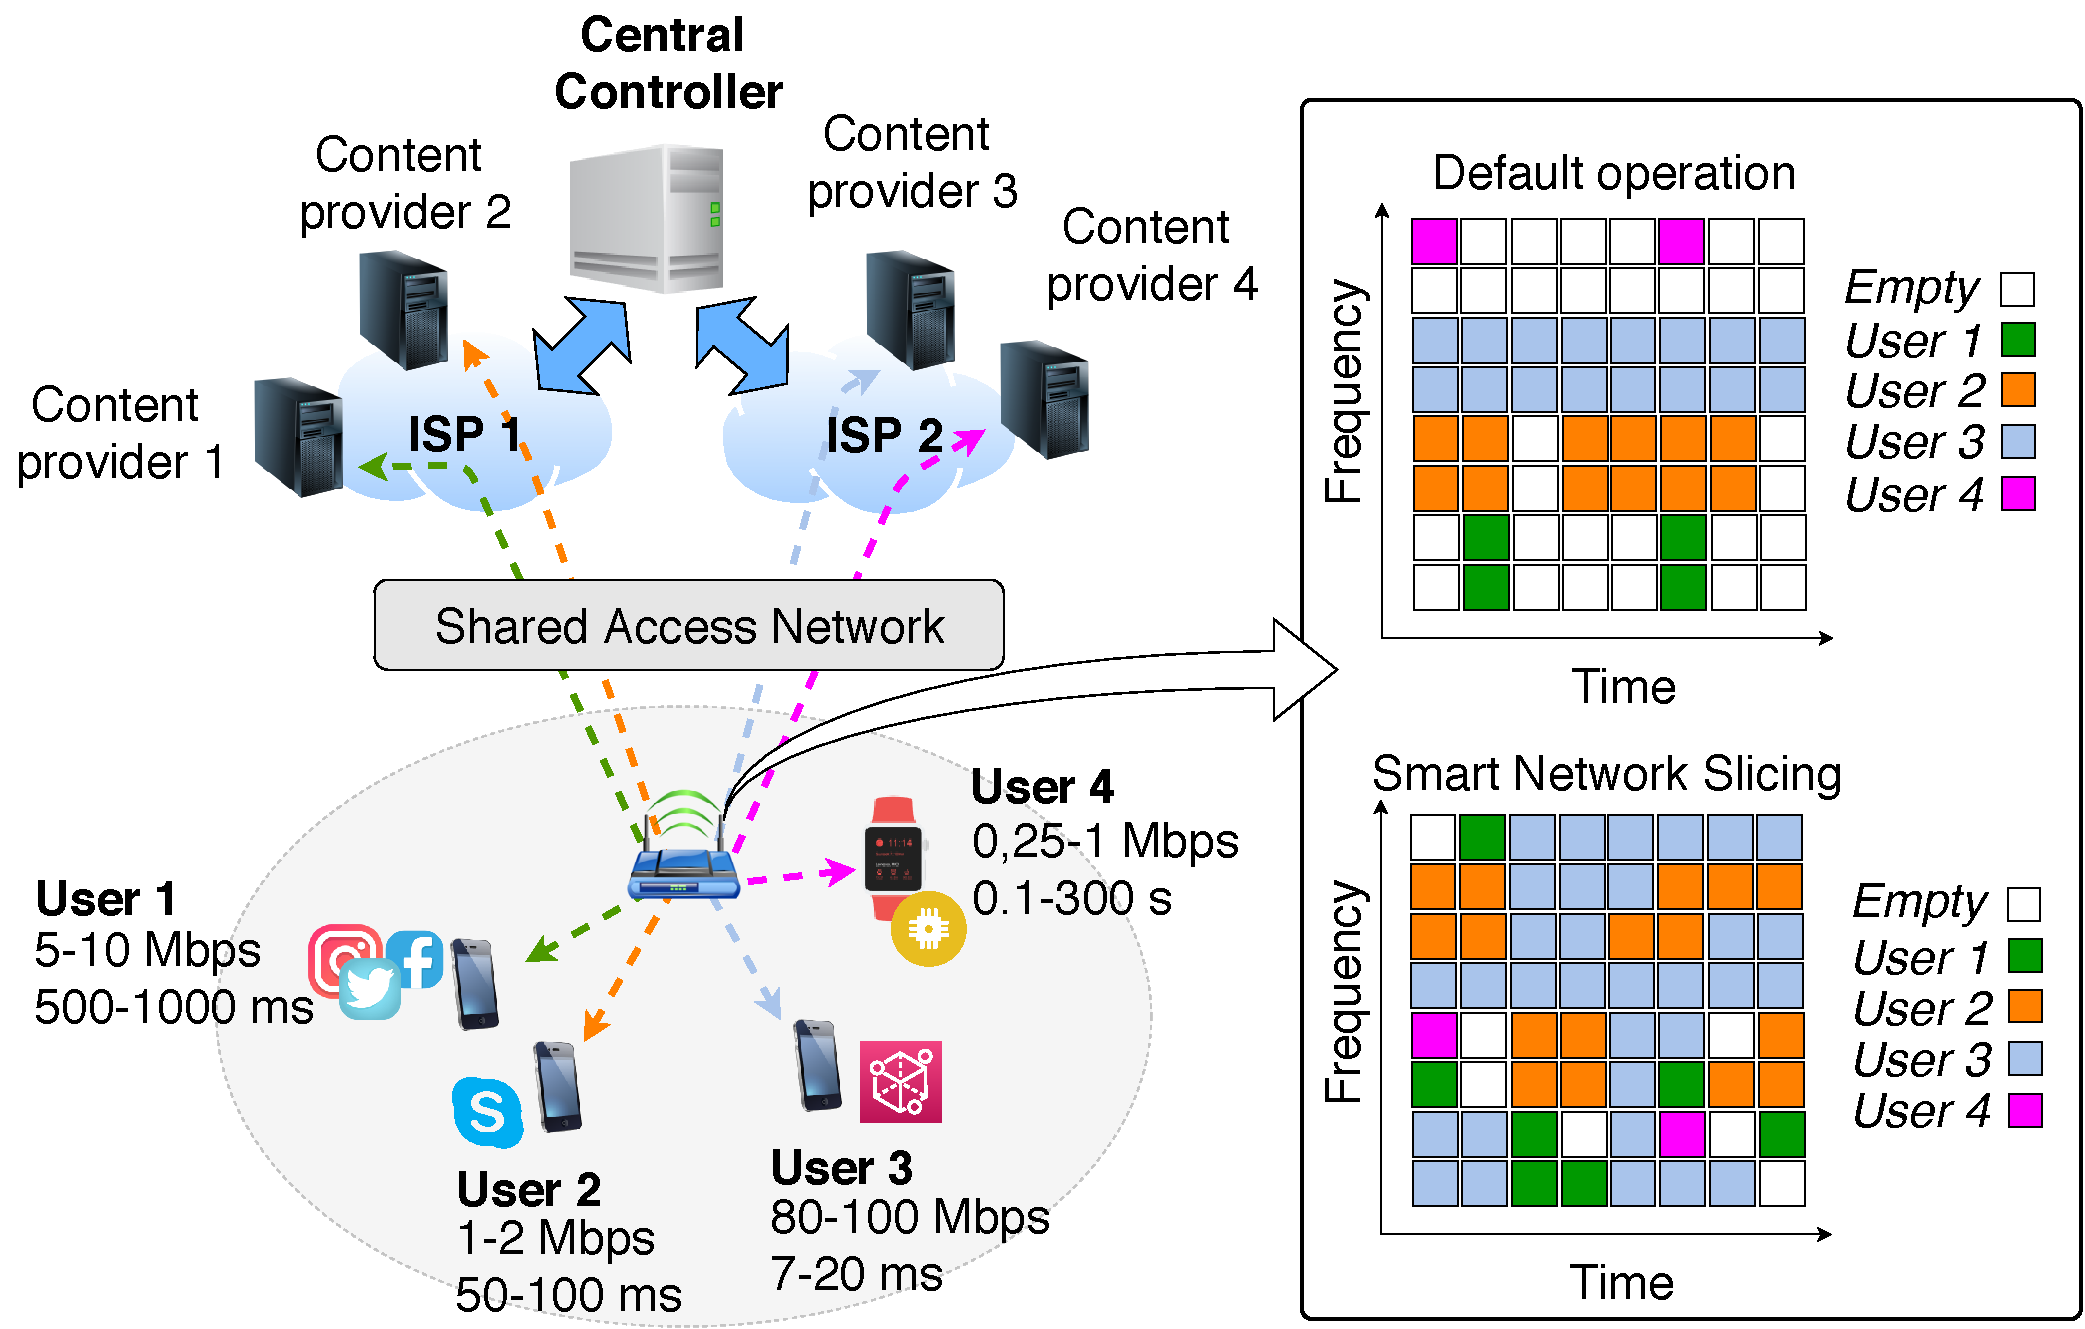
\includegraphics[width=1\columnwidth]{network_slicing_ofdma}
	\caption{OFDMA-based smart network slicing.}
	\label{fig:use_cases}
\end{figure}

\subsubsection{Cloud-Based User Association and Handover}
Most of the current user association and handover procedures held in WLANs typically rely on the Strongest Signal First (SSF) mechanism. This might be problematic in terms of load balancing and can potentially lead to severe performance degradation in dense Basic Service Sets (BSSs). By introducing ML, it is possible to handle contextual information such as the traffic load, which can be useful for decision-making. Furthermore, mobility pattern prediction and user requirements forecasts can be included in the system, thus empowering the association and handover mechanisms with insightful information.

\subsubsection{Inference-Based Coordinated Scheduling}
Contrary to traditional cellular-type networks, WLAN deployments can be chaotic, especially in residential scenarios where anyone can set-up an AP and create a wireless network. This typically leads to complex scenarios where inter-BSS interactions prevent the existing scheduling approaches to ensuring a minimum quality of service. Fortunately, ML can be used to infer these interactions and provide a solution accordingly. In particular, through coordinated ML-assisted scheduling, different APs can trigger uplink/downlink transmissions from/to the appropriate stations (STAs), thus increasing the network throughput whilst reducing the number of packet collisions.

\subsubsection{Reinforcement Learning-Based Spatial Reuse} 
Spatial reuse aims to improve channel utilization through sensitivity adjustment mechanisms. However, selecting the best sensitivity threshold is not trivial given the complex spatial interactions that occur among devices. As a potential solution, reinforcement learning can be applied locally to improve spectral efficiency in a decentralized manner.

% ----------------------------------
% -
% 	-- ITU-T ARCHITECTURE --
% -
% ----------------------------------

\section{ITU Unified Architecture for Future Networks}
\label{section:itu_architecture}

\begin{figure*}[!ht]
	\centering
	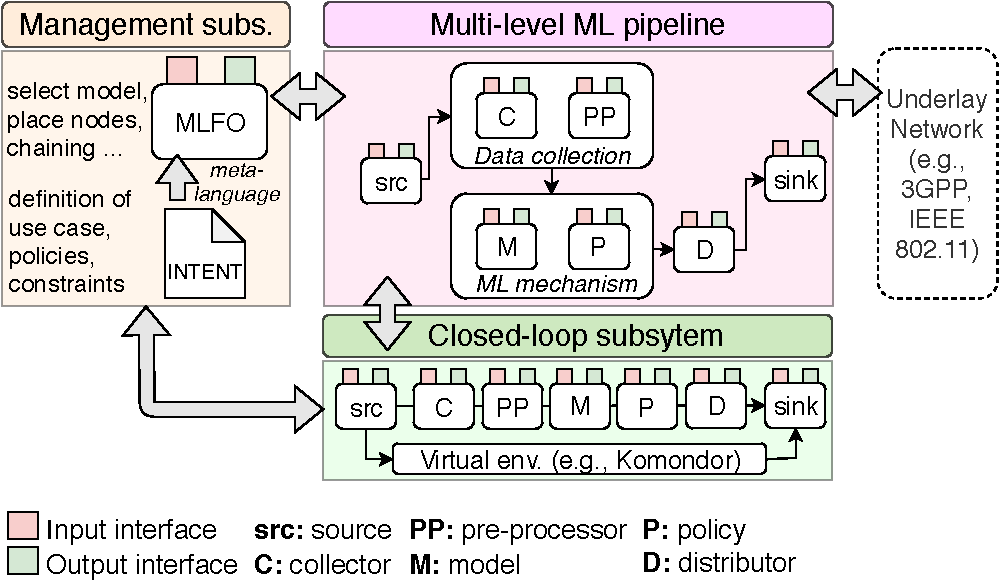
\includegraphics[width=0.55\textwidth]{itu_ml_architecture}
	\caption{ITU's logical architecture for future networks \cite{itu2019architecture}. Entities contain input/output interfaces for communication, while the ML intent is a declarative file with information related to the use case.}
	\label{fig:itu_ml_architecture}
\end{figure*}

The FG-ML5G was created in November 2017 by its parent group, the ITU-T Study Group 13, to study the integration of ML mechanisms into future networks. This includes the definition of interfaces, protocols, data formats, and architectures. During its lifetime, the FG-ML5G has released several reports and contributions. Among them, we highlight the ITU's logical interoperable architecture for future networks \cite{itu2019architecture}, which defines an ML overlay that operates on the top of any unspecified underlay network technology (e.g., 3GPP, EdgeX, IEEE 802.11). The ITU's architecture aims to fulfill a set of technology-agnostic high-level requirements to support ML. For instance, the architecture must be able to support multiple types of data, thus taking advantage of heterogeneous data sources. 

Figure \ref{fig:itu_ml_architecture} shows the elements that compose the ML overlay (management subsystem, multi-level ML pipeline, and closed-loop subsystem). These elements are further described in the following subsections. Based on this standard overlay, ML applications can be instantiated in the logical entities (represented by white boxes).

\subsection{Management Subsystem} 
The management subsystem is in charge of the deployment and the orchestration of the ML services that operate in the underlying network. To that purpose, the Machine Learning Function Orchestrator (MLFO) entity is defined. The MLFO is first instantiated by a declarative intent that uses a meta language. It specifies the ML use case to be applied, including initialization, policies, and constraints. Then, the MLFO initializes the elements of the ML pipeline and monitors their operation during execution.

\subsection{Multi-Level Machine Learning Pipeline} 
The multi-level ML pipeline performs the actual ML operation in a given network underlay and it is in charge of the data collection, model application, and output distribution. The following logical entities compose the ML pipeline:
\begin{itemize}
	\item \textbf{Source (src):} generates data to be used by the ML mechanism.
	\item \textbf{Collector (C):} collects the data generated by sources.
	\item \textbf{Pre-processor (PP):} prepares the data collected for its utilization by the ML mechanism.
	\item \textbf{Model (M):} applies the ML model specified by the intent.
	\item \textbf{Policy (P):} provides a set of constraints and/or guidelines that delimit the behavior of the model.
	\item \textbf{Distributor (D):} spreads the ML output across all the corresponding targets (or sinks).
	\item \textbf{Sink (sink):} applies the ML output that is received from the distributor.
\end{itemize}

\subsection{Closed-loop Subsystem} 
In order to address network dynamics, the ML operation is assisted by a closed-loop subsystem, which can provide information to the system beforehand. As for the ML pipeline, the closed-loop subsystem is orchestrated by the management subsystem. In particular, a sandbox can be formed of real devices (pre-production internal network) or even be virtual (simulator/emulator). Network simulators such as ns-3 and Komondor \cite{barrachina2019komondor} are examples of closed-loop subsystems and can serve two purposes: \emph{i)} generate synthetic data for training, and \emph{ii)} run simulations to validate potential solutions before being applied in production.

% ----------------------------------
% -
% 	-- ML Architecture --
% -
% ----------------------------------
\section{Machine Learning-Aware Architecture for IEEE 802.11 WLANs}
\label{section:wlans_architecture}

Based on their independence degree in terms of management and operation, WLAN deployments can be divided into two main families:
\begin{itemize}
	\item \textbf{Enterprise:} a set of BSSs can be jointly operated from the edge and/or the cloud, thus providing management and orchestration functionalities such as centralized authentication, or channel allocation. Enterprise-like deployments are realized through Extended Service Sets (ESS) and can be typically found in environments controlled by a single network operator, like university campuses, offices, stadiums, etc. 
	\item \textbf{Residential:} each BSS is responsible for its own management and operation. In the context of residential scenarios (but not limited to), peer-to-peer deployments are gaining popularity for infrastructureless communications (e.g., Wi-Fi direct).
\end{itemize}

\begin{figure}[ht!]
	\centering
	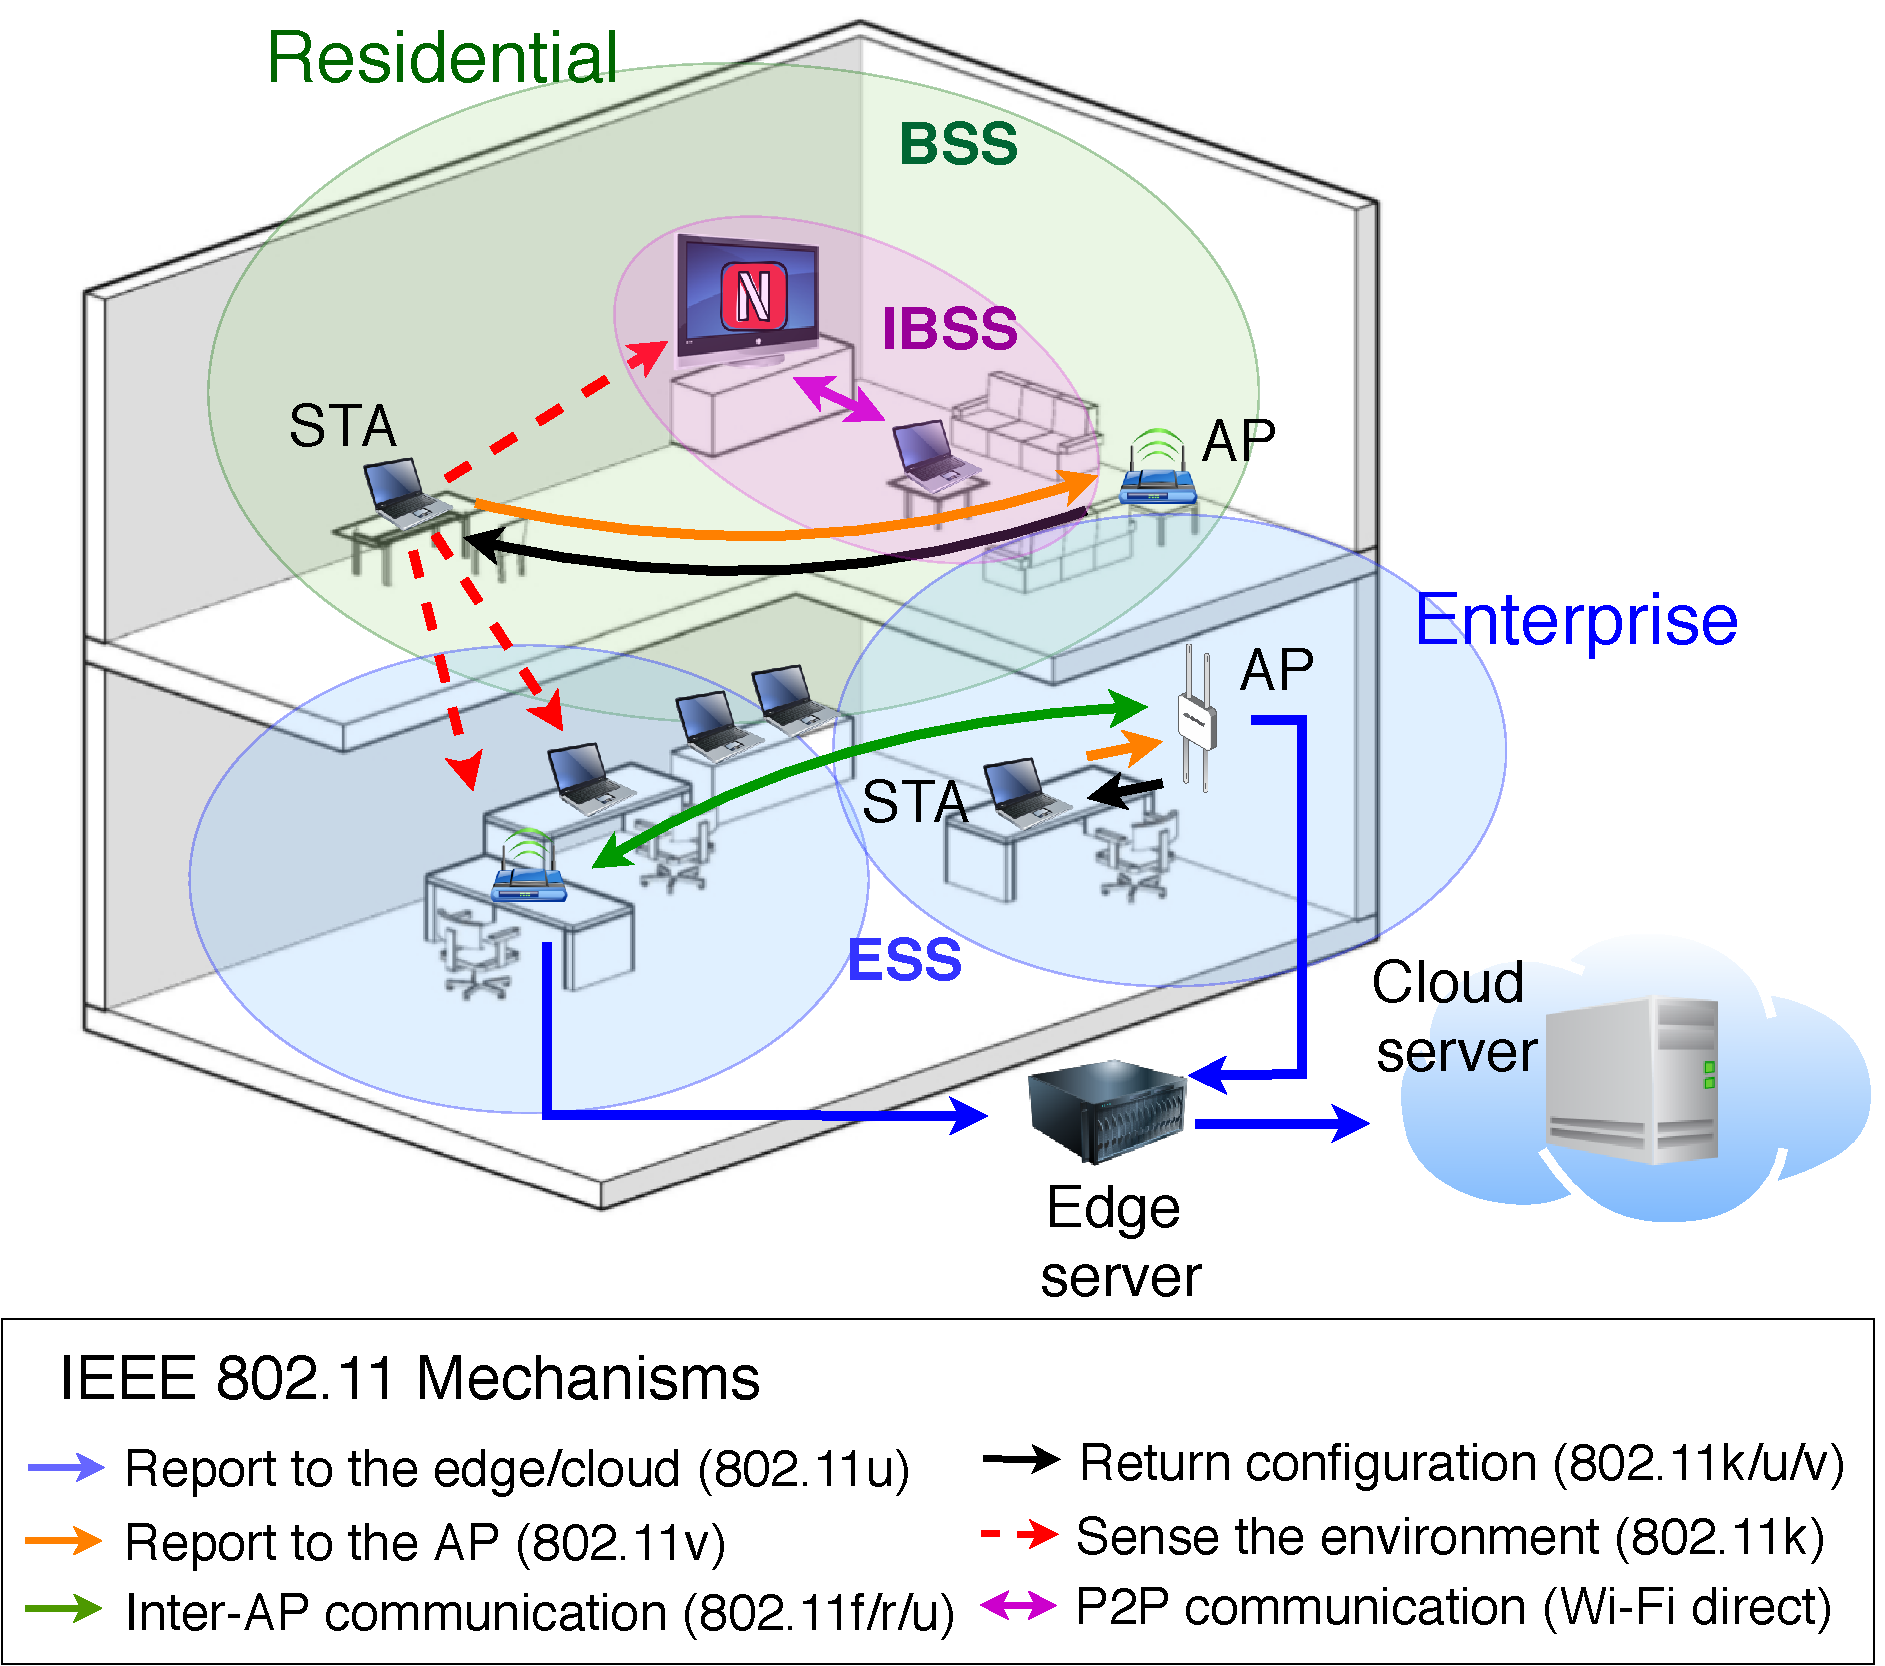
\includegraphics[width=\columnwidth]{overview_learning_approaches}
	\caption{Enterprise and residential-like deployments and complementary IEEE 802.11 mechanisms to enable the utilization of ML.}
	\label{fig:overview_learning_approaches}
\end{figure}

Figure \ref{fig:overview_learning_approaches} illustrates the enterprise and residential-like deployments as well as a set of mechanisms that can facilitate the adoption of the ML-based architecture in WLANs. The following functionalities are provided:
\begin{itemize}
	\item \textbf{Information gathering (802.11k/r/v):} ML mechanisms can use information about the network topology and RF measurements to infer the behavior of other devices, or to extract important environmental characteristics.
	\item \textbf{Interoperability (802.11f/u):} Interoperability enables coordinated operations (e.g., scheduling, resource allocation), thus allowing to apply centralized/coordinated mechanisms such as in federated learning.
	\item \textbf{Security (802.11w):} ML mechanisms can use management frames that are protected so that a higher level of security is granted.
	\item \textbf{Validation (802.11t):} Performance evaluation in WLANs through test metrics can be useful to define optimization goals within the ML  operation.
\end{itemize}

%%% CHALLENGES IN IEEE 802.11 WLANs
\subsection{Challenges in IEEE 802.11 WLANs}
\label{section:ieee_80211_wlans}
The application of ML methods in WLANs is tightly tied to the technological challenges posed by these types of networks. The major challenges encountered in wireless communications stand for fast data expiry and lack of resources for data handling (e.g., storage, computation, and information exchange). Regarding Wi-Fi networks, we find the following challenges:
\begin{enumerate}
	\item \textbf{Non-stationarity:} channel fluctuations due to multipath fading, mobility of users and varying traffic needs entail a big challenge to ML applications. As a result of network dynamics, adaptability should be granted by continuously retraining ML models.
	\item \textbf{Limited communication resources:} since Wi-Fi operates under unlicensed bands, resources are scarce and shared. Hence, any potential communication required by a certain ML mechanism (as for distributed learning) may fail or be delayed if the medium is congested. As a result, the ML operation must be robust and resilient enough to react to potential communication issues.
	\item \textbf{Limited computation and storage resources:} computation and storage resources may also be scarce in WLANs, especially in residential-like deployments. Therefore, the ML operation should include computation-efficient procedures. Another implication of limited resources lies in the availability of information to be used by ML algorithms, especially for online learning methods.
	\item \textbf{Adversarial environment:} in many cases, Wi-Fi deployments are chaotic in the sense that many overlapping BSSs coexist without cooperation. This is a particularly interesting challenge for ML methods, where competition among agents may lead to an adversarial setting. Moreover, multi-vendor devices may implement different ML mechanisms, leading to clashing interests.
	\item \textbf{Legacy devices:} BSSs may coexist with other legacy devices that do not perform any intelligent operation. It is then required for ML methods to be aware of those devices, so that unfair situations are avoided.
\end{enumerate}

Apart from the previous WLAN-specific challenges, other inter-domain issues should be considered. For instance, end-to-end security is required since ML mechanisms store and/or exchange sensitive data that may be exposed. Besides, interoperability should be tackled when deploying ML solutions to different underlay networks. In this regard, the standardized ITU ML pipeline stands up as a promising solution.

%%% REALIZATION OF THE ADOPTED ARCHITECTURE
\subsection{Computation Paradigms in IEEE 802.11 WLANs}
The various types of WLAN deployments and their computation and communication capabilities are closely linked to the type of ML solutions that can be applied to them: \emph{cloud} or \emph{edge-oriented}.

Cloud-oriented ML applications are characterized by
bearing high computational and storage resources, thus allowing them to collect various types of data from multiple sources, and to provide global and long-term solutions. The major challenge for cloud-oriented methods lies in the management of data and the corresponding synchronization, availability, and heterogeneity issues.

In edge-oriented mechanisms, the ML operation is mainly ruled by edge devices (e.g., APs and/or STAs), which, contrary to the cloud approach, typically lack powerful computation and storage resources. In consequence, edge-oriented mechanisms may only allow using simple and lightweight computing ML algorithms. Nevertheless, edge servers can be added to deploy more powerful solutions promptly. The edge-oriented approach is useful for real-time ML applications that manage local (and even highly-varying) information.

Apart from cloud and edge-oriented settings, we may distinguish between methods based on their cooperation degree. In cooperative approaches, nodes interact among them for the sake of jointly conducting the learning operation (e.g., sharing a reward). However, reliable and timely connections among learners are often required. In this regard, \cite{lin2017deep} showed the role of communications on speeding up a distributed training procedure over a set of nodes in a network. Alternatively, for the non-cooperative case, the learning operation may lead to adversarial settings, especially since BSSs share resources such as the spectrum.

\subsection{Realization of the ML-Aware Architecture for WLANs}

To showcase the adoption of the architecture, let us retake the AP (re)association and handover example (see Fig. \ref{fig:ml_architecture_wlan}). We now consider a hybrid solution where two main ML-based processes are held: training (learn from data) and placement (apply the learned knowledge). 

While the training procedure is carried out at the cloud (collect data from multiple sources), the placement operation is done at the edge (provide timely responses to new cases). Notice that the system can also be re-trained during the placement phase, based on newly acquired local data.

\begin{figure}[ht!]
	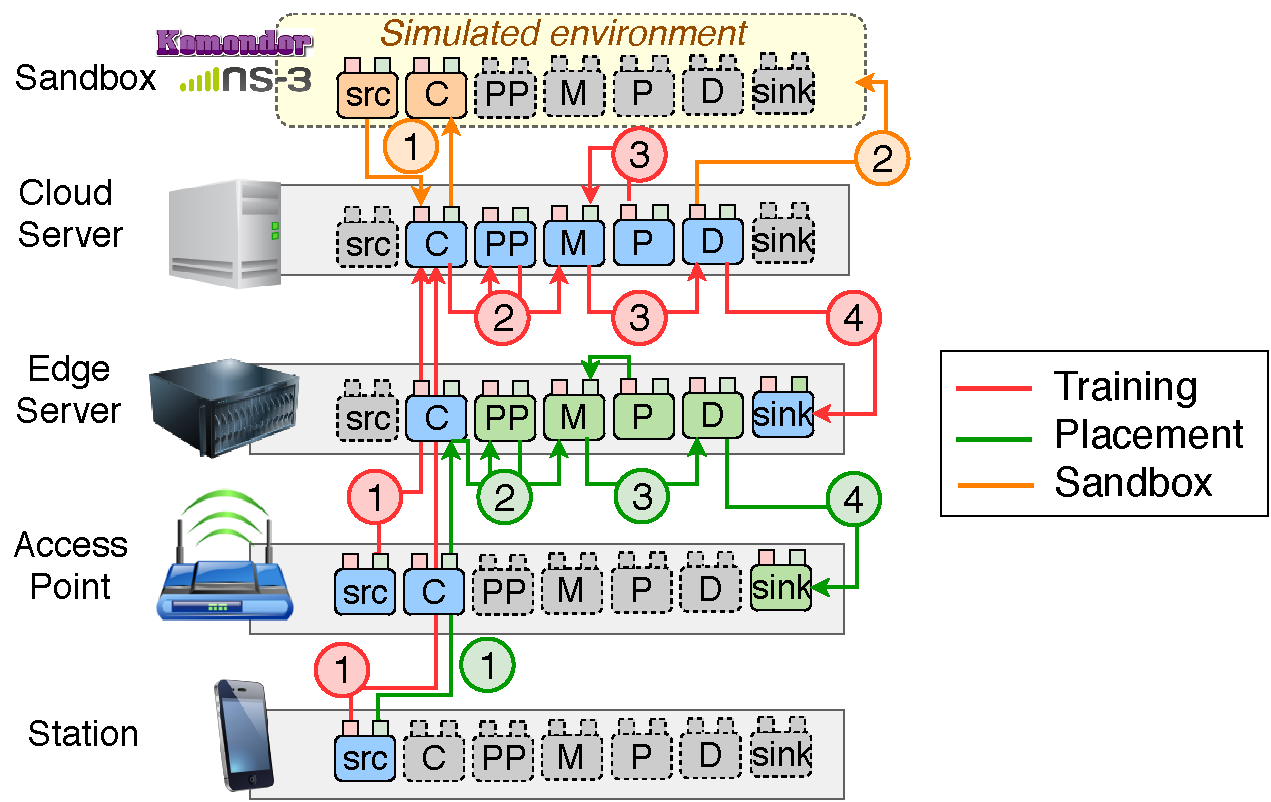
\includegraphics[width=1\columnwidth]{ml_architecture_wlan_2}
	\caption{Realization of the ITU's ML architecture for IEEE 802.11 WLANs through a hybrid ML-based solution for AP (re)association and handover.}
	\label{fig:ml_architecture_wlan}
\end{figure}

Specifically, the training procedure consists of the following steps (shown in red):
\begin{enumerate}
	\item \textbf{Data collection:} the cloud server collects information of different kinds from APs and STAs, such as user information (e.g., location), performance (e.g., delay), application data (e.g., traffic load), or channel status reports (e.g., sensed interference). This information can be used either for training or feeding auxiliary algorithms that help the main AP association procedure (e.g., predict user behavior).
	\item \textbf{Pre-processing:} the data collected at the cloud is pre-processed so that the ML method can properly manage it. For instance, in case of applying a multiple linear regression, the input information needs to be converted into normalized features (i.e., convert the rate given in Mbps into a scalar between 0 and 1).
	\item \textbf{Model generation:} when generating the ML model, certain policies need to be considered. For instance, an AP may set a maximum number of associated STAs. The policies are strongly tied to the capabilities of the devices or the existing regulations (e.g., maximum regulated transmission power).
	\item \textbf{Output distribution:} once the ML method in the cloud generates the output (i.e., the predicted function for new (re)associations), it is distributed throughout the sink edge servers, which are then ready to give quick response to new cases.
\end{enumerate}

In the placement phase (shown in green), we find:
\begin{enumerate}
	\item \textbf{Handle new requests:} new (re)association requests or potential handovers are detected based on newly acquired information from STAs. This information is collected by the edge server.
	\item \textbf{Pre-processing:} the acquired information is then processed by the edge server, just like for the training phase.
	\item \textbf{Run the ML solution:} the ML method provided by the cloud is applied locally at the edge server, which provides an output for the new request.
	\item \textbf{Apply the ML solution:} the (re)association decision is distributed to the corresponding AP.
\end{enumerate}

Finally, it is worth pointing out the role of the sandbox, which can be mainly twofold (shown in orange):
\begin{enumerate}
	\item \textbf{Generate data for training:} the sandbox can act as a source in the ML pipeline by generating synthetic data for training purposes. Nevertheless, the data provided by the sandbox is limited to several factors such as the accuracy of the simulation model or the degree of similarity between the sandbox and the real network. %Also, data collected from the network can be used in the sandbox.
	\item \textbf{Preliminary model testing:} alternatively, the sandbox can be used to validate the output of the ML method before being applied to the real network.
\end{enumerate}

To showcase the potential of the ML-based architecture through numerical results,\footnote{Given the novelty of the technologies studied in this paper, our results have been obtained from well-know standard-compliant models, hence their accuracy is tied to them. Nevertheless, this is a first step to understand the potential benefits of using an ML-based architecture in next-generation wireless networks. For the sake of reproducibility and disclosure, all the source code is open and publicly available at \href{https://github.com/fwilhelmi/machine_learning_aware_architecture_wlans}{https://github.com/fwilhelmi/machine\_learning\_aware\_architecture\_wlans}, accessed January 31, 2020.} we compare the performance of classical AP association procedure (SSF) against a novel ML-based approach (based on vanilla neural networks). In particular, the neural network predicts the throughput that an STA will obtain after associating to a given AP based on a set of features or characteristics (e.g., current load, received signal strength). Figure \ref{fig:results_use_case} shows the throughput received by each STA versus the load it generates, for different deployment densities. We observe that the ML approach improves the average performance and balances the results obtained by all the STAs. This is because the ML function can capture complex patterns from dense deployments, thus guaranteeing minimum throughput requirements to STAs (at the expense of missing the maximum performance peaks).

\begin{figure}[ht!]
	\centering
	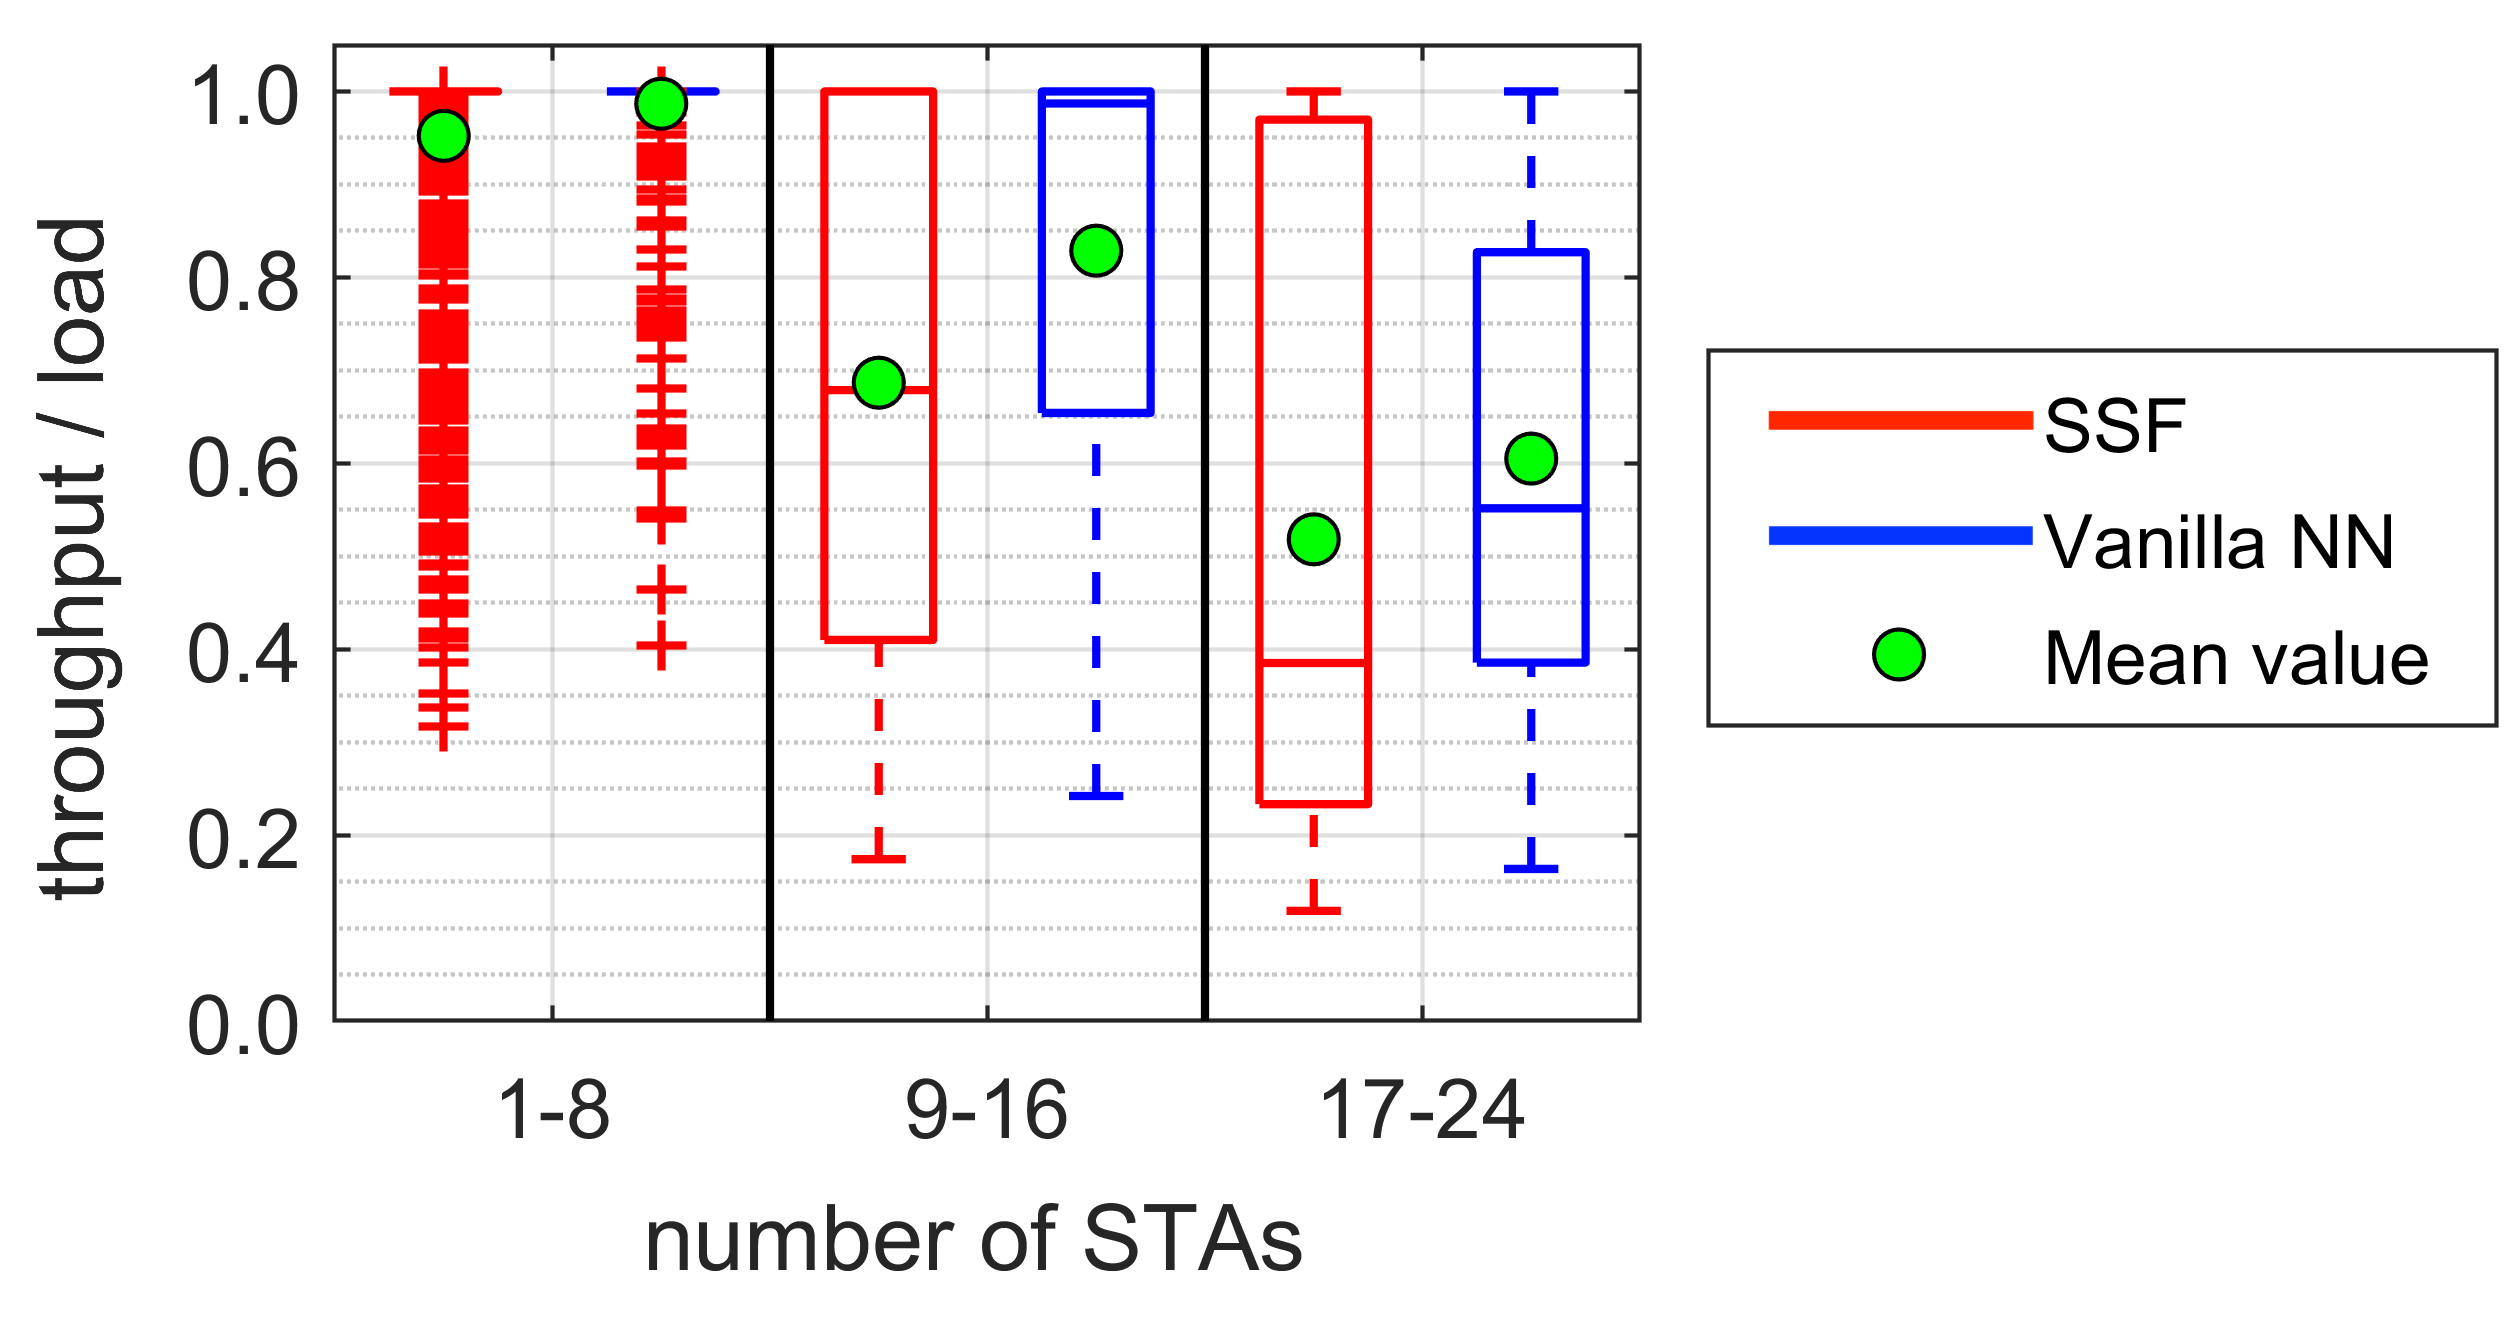
\includegraphics[width=\columnwidth]{output_use_case_ap_association}
	\caption{Performance evaluation of the AP association problem in WLANs: SSF versus Neural Network (NN). The mean performance of each mechanism is represented by a green dot.}
	\label{fig:results_use_case}
\end{figure}

\section{Concluding Remarks}
Current networks are not yet prepared for the pervasive adoption of ML-based operation. Hence, disruptive architectural changes are required. For the sake of moving forward in this field, this article introduced the ITU's unified architecture for future networks and provided a realization for IEEE 802.11 WLANs. The different forms of Wi-Fi networks allow uplifting the flexibility characteristic of the ITU's architecture, thus enabling from edge to cloud-oriented solutions, including hybrid approaches. 

To conclude, future wireless networks are envisioned to share a common flexible architecture that allows a fast adaptation of resources to accommodate a plethora of ML-enabled verticals. Nevertheless, a lot of effort is still required before reaching fully intelligent wireless networks. Among several open issues, we highlight the ones related to data handling (\textit{how/where to store data? how to assess the expiry of data?}), orchestration (\textit{how to distribute the ML operation? how to deal with heterogeneity?}), and robustness of the ML methods (\textit{how to deal with uncertainty? how to prevent unprecedented events}?). 

% use section* for acknowledgment
\section*{Acknowledgment}

This work has been partially supported by grants MDM-2015-0502, 2017-SGR-11888, by WINDMAL PGC2018-099959-B-I00 (MCIU/AEI/FEDER,UE), by a Gift from the Cisco University Research Program (CG\#890107) Fund, and by SPOTS project (RTI2018-095438-A-I00) funded by the Spanish Ministry of Science, Innovation and Universities. The work by Sergio Barrachina-Mu\~noz is supported by an FI grant from Generalitat de Catalunya.

% Can use something like this to put references on a page
% by themselves when using endfloat and the captionsoff option.
\ifCLASSOPTIONcaptionsoff
  \newpage
\fi

% trigger a \newpage just before the given reference
% number - used to balance the columns on the last page
% adjust value as needed - may need to be readjusted if
% the document is modified later
%\IEEEtriggeratref{8}
% The "triggered" command can be changed if desired:
%\IEEEtriggercmd{\enlargethispage{-5in}}

% references section

% can use a bibliography generated by BibTeX as a .bbl file
% BibTeX documentation can be easily obtained at:
% http://mirror.ctan.org/biblio/bibtex/contrib/doc/
% The IEEEtran BibTeX style support page is at:
% http://www.michaelshell.org/tex/ieeetran/bibtex/
\bibliographystyle{IEEEtran}
\bibliography{bibliography}

% if you will not have a photo at all:
\begin{IEEEbiographynophoto}{Francesc Wilhelmi}
(francisco.wilhelmi@upf.edu) holds a B.Sc. degree in Telematics Engineering (2015) and an M.Sc. in Intelligent and Interactive Systems (2016), both from Universitat Pompeu Fabra (UPF). He is currently pursuing a Ph.D. in Information and Communication Technologies at UPF.
\end{IEEEbiographynophoto}

\begin{IEEEbiographynophoto}{Sergio Barrachina-Mu\~noz}
(sergio.barrachina@upf.edu) obtained his B.Sc. degree in Telematics Engineering and his M.Sc. in Intelligent Interactive Systems in 2015 and 2016, respectively, both from Universitat Pompeu Fabra (UPF), Barcelona. Currently, he is a PhD student and teacher assistant in the Wireless Networking research group at UPF.
\end{IEEEbiographynophoto}

\begin{IEEEbiographynophoto}{Boris Bellalta}
(boris.bellalta@upf.edu) is an Associate Professor in the Department of Information and Communication Technologies (DTIC) at Universitat Pompeu Fabra (UPF). He is the head of the Wireless Networking research group at DTIC/UPF.
\end{IEEEbiographynophoto}

\begin{IEEEbiographynophoto}{Cristina Cano}
(ccanobs@uoc.edu) holds a Ph.D. (2011) in Information, Communication and Audiovisual Media Technologies from Universitat Pompeu Fabra (UPF). She has been a research fellow in the Hamilton Institute of the National University of Ireland, Maynooth (2012-2014), in Trinity College Dublin (2015-2016) and in Inria-Lille in France (first half of 2016). Currently, she is an associate professor at Universitat Oberta de Catalunya (UOC). 
\end{IEEEbiographynophoto}

\begin{IEEEbiographynophoto}{Anders Jonsson}
(anders.jonsson@upf.edu) is the director of the Artificial Intelligence and Machine Learning group at Universitat Pompeu Fabra (UPF). He received his Ph.D. in computer science in 2005 from the University of Massachusetts Amherst, USA, and has been at UPF ever since.
\end{IEEEbiographynophoto}

\begin{IEEEbiographynophoto}{Vishnu Ram}
(vishnu.n@ieee.org) worked for Motorola/Nokia/Siemens in advanced technologies teams for 21 years. He was a Scientific Advisory Board Associate (SABA) member of Motorola Networks. He has published several drafts in IETF, contributed to ETSI, 3GPP in his role as a senior specialist (Radio Resource Management). He is currently working as an independent researcher.	
\end{IEEEbiographynophoto}

\vfill

% You can push biographies down or up by placing
% a \vfill before or after them. The appropriate
% use of \vfill depends on what kind of text is
% on the last page and whether or not the columns
% are being equalized.

%\vfill

% Can be used to pull up biographies so that the bottom of the last one
% is flush with the other column.
%\enlargethispage{-5in}

% that's all folks
\end{document}